%% FullCourse_10Lecs -- Lecture 3, Topic 3.1: Why ML + Pattern Recognition
%% Source: ./archive_pre_split/Lec03_ML_for_Macro.tex (sections 1-2)

%% Shared preamble for the FullCourse_10Lecs topic decks.
%%
%% Each topic .tex \input's this file, then defines its own \title, \date
%% override (if any), \graphicspath, and \begin{document}.
%%
%% Reconstructed verbatim from the inlined copy preserved in
%% Lec10_Case_Studies/Lec10_T8_Case6_DeepRamsey.tex (lines 23-190), which is
%% explicitly annotated there as "from ../shared_preamble.tex, copied verbatim".
%% Base preamble matches MiniCourse_8hr/Slides/shared_preamble.tex; this version
%% additionally provides \sectiondivider, the conceptbox/cautionbox/examplebox/
%% takeawaybox tcolorboxes, and \compacttables used across the split decks.

\documentclass[10pt,english,aspectratio=169]{beamer}

\usepackage{ae,aecompl}
\usepackage[T1]{fontenc}
\usepackage{textcomp}
\usepackage[utf8]{inputenc}
\usepackage{babel}
\usepackage{datetime2}

\setcounter{secnumdepth}{3}
\setcounter{tocdepth}{3}

\usepackage{amsmath, amssymb, amsthm, graphicx}
\usepackage{booktabs, multirow}
\usepackage{tikz}
\usepackage{pgfplots}
\pgfplotsset{compat=1.16}
\usepackage[most]{tcolorbox}
\tcbuselibrary{skins, breakable, theorems}
\usepackage{listings}
\usepackage{xcolor}

\lstset{
  basicstyle=\ttfamily\small,
  keywordstyle=\color{blue!80!black}\bfseries,
  commentstyle=\color{green!50!black}\itshape,
  stringstyle=\color{orange!80!black},
  backgroundcolor=\color{gray!8},
  frame=single,
  rulecolor=\color{gray!40},
  breaklines=true,
  showstringspaces=false,
  numbers=none,
}

\lstdefinestyle{pythonstyle}{
    language=Python,
    basicstyle=\ttfamily\footnotesize,
    keywordstyle=\color{blue!80!black}\bfseries,
    commentstyle=\color{green!50!black}\itshape,
    stringstyle=\color{orange!80!black},
    frame=single,
    breaklines=true,
    showstringspaces=false,
    numbers=left,
    numbersep=5pt,
    numberstyle=\tiny\color{gray},
    backgroundcolor=\color{gray!8},
    rulecolor=\color{gray!40}
}

\ifx\hypersetup\undefined
  \AtBeginDocument{%
    \hypersetup{bookmarks=false,breaklinks=true,pdfborder={0 0 0},colorlinks=true,
      linkcolor=DarkText,urlcolor=RedTitle}%
  }
\else
  \hypersetup{bookmarks=false,breaklinks=true,pdfborder={0 0 0},colorlinks=true,
    linkcolor=DarkText,urlcolor=RedTitle}%
\fi

\makeatletter
\newcommand\makebeamertitle{%
  \begin{frame}[plain]
    \vspace*{1.0cm}
    \centering
    {\usebeamerfont{title}\usebeamercolor[fg]{title}\inserttitle\par}
    \vspace{1.0cm}
    {\usebeamerfont{author}\usebeamercolor[fg]{author}\insertauthor\par}
    \vspace{0.2cm}
    {\usebeamerfont{date}\usebeamercolor[fg]{date}\insertdate\par}
  \end{frame}}%
\AtBeginDocument{%
  \let\origtableofcontents=\tableofcontents
  \def\tableofcontents{\@ifnextchar[{\origtableofcontents}{\gobbletableofcontents}}
  \def\gobbletableofcontents#1{\origtableofcontents}%
}

\usetheme{metropolis}
\usefonttheme{professionalfonts}

\definecolor{LightGray}{RGB}{230,230,230}
\definecolor{RedTitle}{RGB}{0,0,200}
\definecolor{VeryLightGray}{RGB}{245,245,245}
\definecolor{DarkText}{RGB}{0,0,0}

\setbeamercolor{background canvas}{bg=white}
\setbeamercolor{title}{fg=RedTitle}
\setbeamercolor{author}{fg=DarkText}
\setbeamercolor{date}{fg=DarkText}
\setbeamercolor{frametitle}{bg=VeryLightGray,fg=DarkText}
\setbeamercolor{normal text}{fg=DarkText}
\setbeamerfont{title}{size=\large}

\setbeamersize{text margin left=5mm, text margin right=5mm}
\addtobeamertemplate{frametitle}{}{\vspace{-0.5em}}
\newcommand{\reducevspace}{\vspace{-0.5cm}}

% Shared section divider and box styles for split topic decks.
\newcommand{\sectiondivider}[2]{%
\begin{frame}[plain,noframenumbering]
\begin{center}
\vfill
{\Large\textbf{#1}\par}
\vspace{0.35cm}
{\normalsize #2\par}
\vfill
\end{center}
\end{frame}
}

\newtcolorbox{conceptbox}[1][]{
  colback=blue!3,
  colframe=RedTitle!55,
  boxrule=0.35mm,
  arc=1mm,
  left=2mm,
  right=2mm,
  top=1mm,
  bottom=1mm,
  #1
}
\newtcolorbox{cautionbox}[1][]{
  colback=red!3,
  colframe=red!50!black,
  boxrule=0.35mm,
  arc=1mm,
  left=2mm,
  right=2mm,
  top=1mm,
  bottom=1mm,
  #1
}
\newtcolorbox{examplebox}[1][]{
  colback=green!3,
  colframe=green!45!black,
  boxrule=0.35mm,
  arc=1mm,
  left=2mm,
  right=2mm,
  top=1mm,
  bottom=1mm,
  #1
}
\newtcolorbox{takeawaybox}[1][]{
  colback=VeryLightGray,
  colframe=RedTitle!55,
  boxrule=0.35mm,
  arc=1mm,
  left=2mm,
  right=2mm,
  top=1mm,
  bottom=1mm,
  #1
}
\newcommand{\compacttables}{\renewcommand{\arraystretch}{1.15}}

\setbeamertemplate{navigation symbols}{}
\setbeamertemplate{footline}{%
  \hfill%
  \usebeamercolor[fg]{page number in head/foot}%
  \usebeamerfont{page number in head/foot}%
  \insertframenumber\,/\,\inserttotalframenumber\kern1em\vskip2pt%
}

\makeatother

\author{Zhigang Feng}
% "date with time": compile timestamp so each build is identifiable.
\date{\today\ \DTMcurrenttime}


\graphicspath{{./pic/}{../../MiniCourse_8hr/Slides/Module1_ML_Foundations/pic/}{../}}

% Suppress the redundant auto-generated metropolis section page; the
% \sectiondivider frames below are the dividers we keep.
\metroset{sectionpage=none}
\usetikzlibrary{positioning,arrows.meta,shapes,calc}
%% Lec03 shared MAP slide: "one map, four acts" recurring diagram.
%% Input this file AFTER ../shared_preamble.tex (needs RedTitle, VeryLightGray,
%% DarkText) and AFTER \usetikzlibrary{positioning,arrows.meta,shapes,calc}.
%% Call \LecThreeMap{k} inside a frame, where k in {1,2,3,4} highlights the
%% current act ("you are here") and k = 0 renders the closing reprise with all
%% four acts checked green (used by T4's closing frame).
%% Filename deliberately does NOT match the build glob Lec*_T*.tex, so the build
%% script never tries to compile it standalone.
%%
%% The four acts are the lecture's story: WHY -> BUILD -> TRAIN -> SHAPE, i.e.
%% the case for ML in economics, the network as an object (architecture + UAT),
%% the learning machinery (backprop + SGD + regularization + double descent),
%% and economics-aware architectures with the hands-on lab.

\newcommand{\LecThreeMap}[1]{%
% Precompute per-box style selectors; TikZ option lists are comma-split before
% TeX conditionals run, so \ifnum must not sit inside a [...] options list.
\ifnum#1=0
  \tikzset{lmapa/.style={lmapdone}, lmapb/.style={lmapdone},
           lmapc/.style={lmapdone}, lmapd/.style={lmapdone}}%
\else
  \tikzset{lmapa/.style={}, lmapb/.style={}, lmapc/.style={}, lmapd/.style={}}%
  \ifnum#1=1 \tikzset{lmapa/.style={lmapcur}}\fi
  \ifnum#1=2 \tikzset{lmapb/.style={lmapcur}}\fi
  \ifnum#1=3 \tikzset{lmapc/.style={lmapcur}}\fi
  \ifnum#1=4 \tikzset{lmapd/.style={lmapcur}}\fi
\fi
\begin{center}
\begin{tikzpicture}[
    act/.style={rectangle, rounded corners, draw=black!60, fill=VeryLightGray,
        minimum width=3.0cm, minimum height=0.95cm, text width=2.9cm,
        align=center, font=\small, text=DarkText},
    lmapcur/.style={draw=RedTitle, very thick, fill=orange!20},
    lmapdone/.style={draw=green!45!black, thick, fill=green!10},
    q/.style={font=\tiny\itshape, text width=3.0cm, align=center, text=black!70},
    barlab/.style={font=\tiny\bfseries, text=black!65},
    sat/.style={rectangle, rounded corners, draw=black!45, dashed, fill=white,
        text width=5.2cm, align=center, font=\tiny, text=black!70,
        minimum height=0.5cm},
    arr/.style={-{Stealth[length=2.2mm]}, thick, gray!60}
]
    % --- four act boxes ---
    \node[act, lmapa] (a1) at (0,0)
        {\textbf{3.1\ \ WHY}\\[1pt] \tiny the case for ML in econ};
    \node[act, lmapb] (a2) at (3.6,0)
        {\textbf{3.2\ \ BUILD}\\[1pt] \tiny neurons $\cdot$ activations $\cdot$ UAT};
    \node[act, lmapc] (a3) at (7.2,0)
        {\textbf{3.3\ \ TRAIN}\\[1pt] \tiny backprop $\cdot$ SGD $\cdot$ dbl.\ descent};
    \node[act, lmapd] (a4) at (10.8,0)
        {\textbf{3.4\ \ SHAPE}\\[1pt] \tiny ICNN $\cdot$ monotone $\cdot$ lab};
    \draw[arr] (a1) -- (a2);
    \draw[arr] (a2) -- (a3);
    \draw[arr] (a3) -- (a4);
    % --- the student question each act answers ---
    \node[q] at (0,-0.95)    {why should an economist\\ care about ML?};
    \node[q] at (3.6,-0.95)  {what is a neural network,\\ and why does it work?};
    \node[q] at (7.2,-0.95)  {how does it learn ---\\ and why not overfit?};
    \node[q] at (10.8,-0.95) {how do I build economics\\ in --- and run it myself?};
    % --- "you are here" marker above the current act ---
    \ifnum#1=1 \node[font=\scriptsize\bfseries, text=RedTitle] at (0,0.98)
        {you are here\ $\blacktriangledown$};\fi
    \ifnum#1=2 \node[font=\scriptsize\bfseries, text=RedTitle] at (3.6,0.98)
        {you are here\ $\blacktriangledown$};\fi
    \ifnum#1=3 \node[font=\scriptsize\bfseries, text=RedTitle] at (7.2,0.98)
        {you are here\ $\blacktriangledown$};\fi
    \ifnum#1=4 \node[font=\scriptsize\bfseries, text=RedTitle] at (10.8,0.98)
        {you are here\ $\blacktriangledown$};\fi
    \ifnum#1=0 \node[font=\scriptsize\bfseries, text=green!45!black] at (5.4,0.98)
        {all four acts complete};\fi
    % --- bottom band: the ML pipeline (the technical spine of the lecture) ---
    \fill[blue!10]   (-1.55,-1.72) rectangle (5.15,-1.40);
    \fill[green!12]  (5.65,-1.72)  rectangle (8.75,-1.40);
    \fill[orange!16] (9.25,-1.72)  rectangle (12.35,-1.40);
    \node[barlab] at (1.8,-1.56)  {REPRESENT\ (UAT $\cdot$ Barron)};
    \node[barlab] at (7.2,-1.56)  {OPTIMIZE\ (loss $\cdot$ gradient)};
    \node[barlab] at (10.8,-1.56) {GENERALIZE $+$ CONSTRAIN};
    % --- dashed satellites: where this lecture sits in the course flow ---
    \node[sat] at (1.5,-2.42)
        {\textit{upstream:} Lec01--02 --- AI as cognitive capital; deep learning as the engine of the predictive stack};
    \node[sat] at (9.3,-2.42)
        {\textit{downstream:} Lec04--06 --- these networks become Bellman/Euler solvers for dynamic macro models};
\end{tikzpicture}
\end{center}
}


\title[AI for Econ Research]{AI for Economic Research: Dynamic Models, Language, and Agents\\
Lecture 3.1: Why ML for Economists \& Pattern Recognition}

\begin{document}

\makebeamertitle

%=============================================================================
\begin{frame}{Lecture 3 in One Map}
\textbf{One lecture, four decks, one goal: make neural networks a working tool for economists --- why they matter, what they are, how they learn, and how to make them respect economics.}

\LecThreeMap{1}

\vspace{0.05cm}
\footnotesize\textit{\textbf{Act 3.1 (here)} makes the case for ML in economic research --- unstructured data, better prediction and controls, high-dimensional models --- then builds the core intuition with pattern recognition: digits live on a low-dimensional manifold, and networks learn the encoder.}
\end{frame}

%=============================================================================
\section{Why ML for Economists?}

\sectiondivider{Why ML for Economists?}{Four doors ML opens: unstructured data, causal inference, forecasting, and high-dimensional models}

\begin{frame}{Harnessing the Power of Unstructured Data}
\begin{itemize}
\item Economics has traditionally relied on structured, tabular data. However, a wealth of economic information is locked in unstructured formats: text, images, satellite imagery.
\item ML algorithms, particularly deep learning, provide tools to systematically process and quantify this unstructured data into economic indicators.
\item \textbf{Applications:}
\begin{itemize}
\item Measuring economic sentiment and uncertainty from financial news and social media
\item Analyzing satellite images to track economic activity (nighttime lights $\approx$ GDP proxy, ships in ports $\approx$ trade flows)
\item Using image recognition on product pictures to understand non-standardized product features
\end{itemize}
\item \textbf{Course arc:} Lec.\ 1 T1 framed AI as cognitive capital --- the \emph{why}. This lecture delivers the \emph{what} (NN architectures, training algorithms); Lec.\ 4 delivers the \emph{how} (solving dynamic equilibrium models).
\end{itemize}
\end{frame}

\begin{frame}{Extracting Insights from Textual Data}
\begin{itemize}
\item Natural Language Processing (NLP) offers powerful techniques to analyze large volumes of text --- going beyond simple word counts.
\item \textbf{Applications:}
\begin{itemize}
\item Gauging dovish or hawkish stance of central bankers from public communications
\item Identifying key risk factors from corporate annual reports
\item Quantifying the evolution of economic policy uncertainty from news articles
\end{itemize}

\medskip
\item \textbf{For macro:} FOMC minutes, Beige Books, and congressional records contain rich information that traditional econometrics cannot easily exploit.
\end{itemize}
\end{frame}

\begin{frame}{Enhancing Causal Inference and Forecasting}
\begin{itemize}
\item \textbf{Causal Inference:}
\begin{itemize}
\item ``Double Machine Learning'' allows flexible inclusion of high-dimensional controls, reducing omitted variable bias
\item ML identifies \emph{heterogeneous treatment effects}: how does a policy impact vary across subgroups?
\end{itemize}

\medskip
\item \textbf{Forecasting \& Nowcasting:}
\begin{itemize}
\item ML captures complex, non-linear relationships that time-series models miss
\item Regularization (e.g., LASSO) enables ``kitchen sink'' regression without overfitting
\item Nowcasting: real-time economic indicators from credit card transactions, web searches, satellite imagery
\end{itemize}
\end{itemize}
\end{frame}

\begin{frame}{Solving Large-Scale Macro and Finance Models}
\begin{itemize}
\item Cutting-edge models (heterogeneous agents, portfolio choice) feature:
\begin{itemize}
\item High dimensionality and complex non-linear dynamics
\item Traditional grid-based methods hit the \textbf{curse of dimensionality}
\end{itemize}

\medskip
\item ML techniques provide powerful new numerical methods:
\begin{itemize}
\item \textbf{Deep learning:} parameterize policy/value functions with neural networks
\item \textbf{Reinforcement learning:} solve sequential decision problems via simulation
\end{itemize}

\medskip
\item \textbf{Examples:}
\begin{itemize}
\item Optimal fiscal/monetary policy in heterogeneous agent models
\item Life-cycle portfolio choice with realistic income uncertainty
\item Krusell--Smith (1998) with neural network approximation of the law of motion
\end{itemize}
\end{itemize}
\end{frame}

\begin{frame}{ML and the Curse of Dimensionality in Macro}
\begin{itemize}
\item \textbf{CoD \#1: Dimension of the state space}
\begin{itemize}
\item $k\rightarrow\{k,a,h,\ldots\}$; the distribution $\Gamma$ is infinite-dimensional
\item \textit{Traditional:} sparse grids, local approximation --- scale poorly
\item \textit{ML:} neural networks are \textbf{grid-free}; recover equilibrium functions via Monte Carlo sampling
\end{itemize}

\medskip
\item \textbf{CoD \#2: Unfolding of uncertainty}
\begin{itemize}
\item $\mathbb{E}$ over future contingencies; the space for $\Gamma$ is unknown
\item \textit{Traditional:} discretize shocks, impose Markov structure
\item \textit{ML:} focus on the ergodic distribution; direct simulation Monte Carlo
\end{itemize}

\medskip
\item \textbf{Key insight:} ML shifts the computational bottleneck from \emph{grid construction} to \emph{function representation} --- a much more scalable paradigm.

\medskip
\item \textbf{Where this gets concrete in the course:} Lec.\ 4 T1 applies it to the optimal-growth state $(k,z)$; Lec.\ 5 T1 generalizes to MDPs $(S, A, P, R, \gamma)$; Lec.\ 6 attacks high-dim Aiyagari and Krusell--Smith with the methods you'll learn in T2--T4.
\end{itemize}
\end{frame}

%=============================================================================
\section{Pattern Recognition as Motivating Illustration}

\sectiondivider{Pattern Recognition as Motivating Illustration}{Digits, manifolds, encoders --- the intuition behind every network in this course}

\begin{frame}{Example: Handwritten Digit Recognition}
\begin{center}
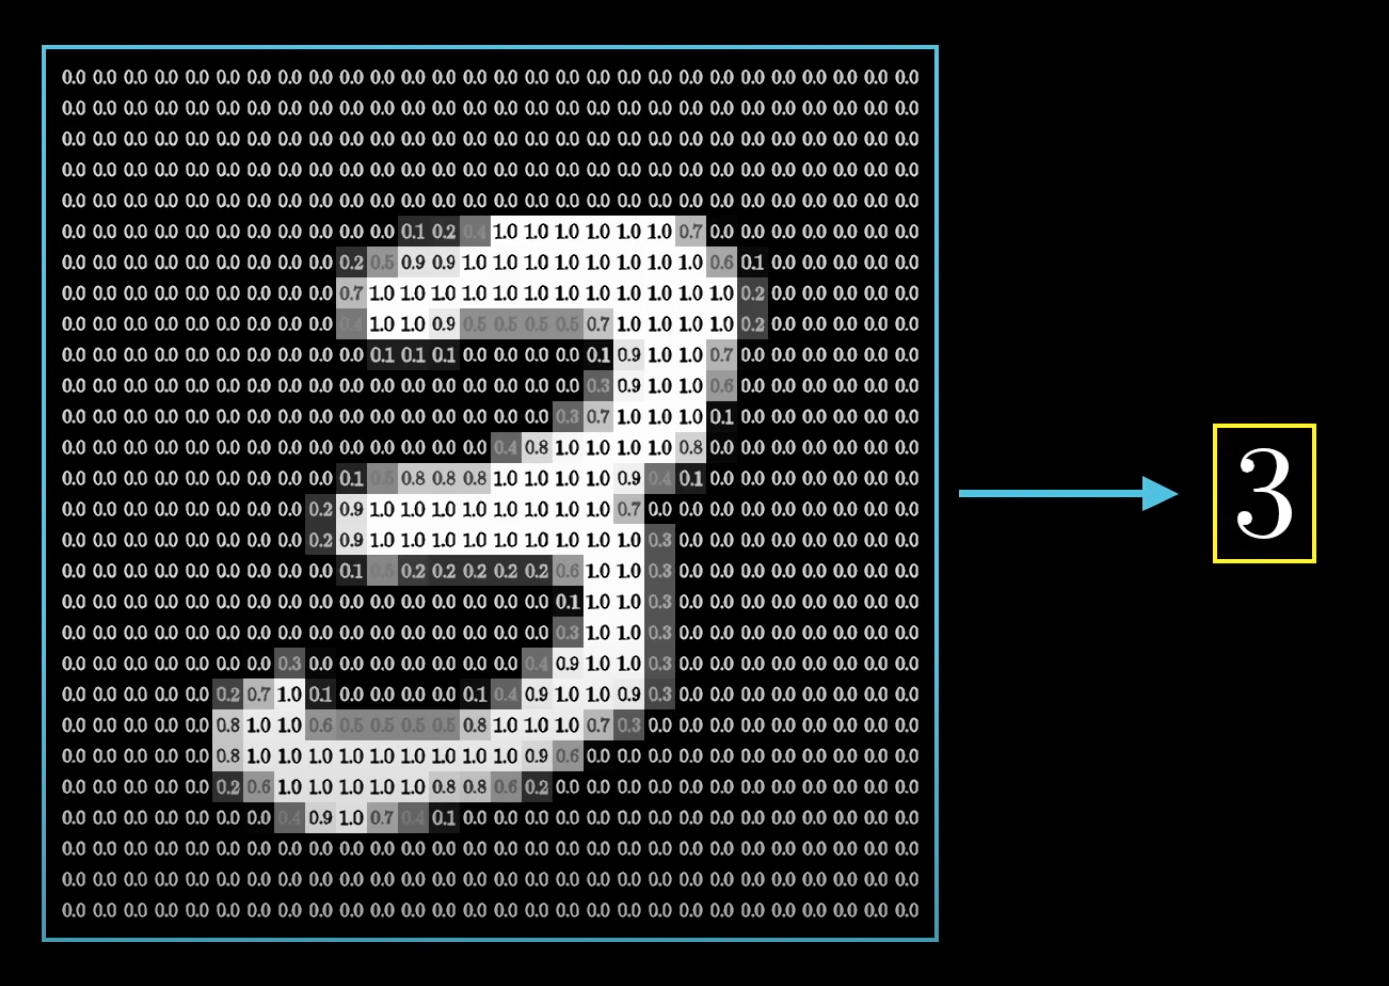
\includegraphics[width=12cm,height=7cm,keepaspectratio]{3.png}
\end{center}
\end{frame}

\begin{frame}{Digit Recognition as a Mathematical Problem}
\begin{itemize}
  \item \textbf{Dataset:}
        $\bigl\{(\mathbf{x}_i, y_i)\bigr\}_{i=1}^N$ with images $\mathbf{x}_i \in [0,1]^{784}$
        and labels $y_i \in \{0,\dots,9\}$

  \item \textbf{Input--Output Mapping:}
        \[
          f_{\theta} \colon \mathbf{x} \longmapsto \hat{\mathbf{p}} \in \Delta^{9},
          \qquad
          \hat{y} = \arg\max_{k} \hat{p}_k
        \]
        where $\Delta^{9}$ is the 10-dimensional probability simplex

  \item \textbf{Learning Objective (Empirical Risk + Regularization):}
        \[
          \min_{\theta} \;
          \frac{1}{N}\sum_{i=1}^{N}
          \underbrace{\mathcal{L}\bigl(f_{\theta}(\mathbf{x}_i), y_i\bigr)}_{\text{cross-entropy}}
          + \lambda \lVert\theta\rVert_{p}
        \]

  \item \textbf{Search Strategy:} Stochastic gradient descent \& variants (Adam, RMSProp)
\end{itemize}
\end{frame}

\begin{frame}{Constraints and Structure in Handwritten Digits}
\begin{itemize}
\item \textbf{Anatomical constraints:} Muscles, tendons, and joints dictate possible strokes --- leading to systematic patterns in how digits are formed.

\medskip
\item \textbf{Geometric properties:} Each digit has defining features --- `0' has a closed loop, `1' a vertical stroke, `8' two stacked loops.

\medskip
\item \textbf{Spatial relationships:} Relative positions, sizes, and orientations of components maintain digit identity even with individual variation.

\medskip
\item \textbf{Lesson for economists:} Just as economic theory constrains the space of plausible models, structural constraints on handwriting reduce the effective dimensionality of the recognition problem.

\medskip
\item ML algorithms can \textbf{learn} these constraints from data --- data augmentation, regularization, and architecture choices all exploit this structure.
\end{itemize}
\end{frame}

\begin{frame}{From 784 Pixels to a Low-Dimensional Manifold}
\begin{itemize}
  \item \textbf{Manifold Hypothesis:}
        Natural digit images occupy a smooth, $d$-dimensional manifold
        $\mathcal{M}\subset\mathbb{R}^{784}$ with $d\ll784$.

  \medskip
  \item \textbf{Plain-English version:} only a few ``writing-style'' degrees of freedom matter:
        slant, stroke thickness, loop closure, and local translation.

  \medskip
  \item The other 780+ pixel directions are nearly empty: random pixel noise almost never looks like a digit.

  \medskip
  \item \textbf{Macro analogy:} finding a low-dimensional state in a high-dimensional model is the same problem.
        A good representation preserves the few variables that matter for the next decision.
\end{itemize}
\end{frame}

\begin{frame}{Encoder View of Digit Recognition}
\begin{itemize}
  \item \textbf{Two-stage model:}
        \[
          \mathbf{x}
          \xrightarrow{\;\pi\,:\;\mathbb{R}^{784}\!\!\to\mathbb{R}^{d}\;}
          \mathbf{z}
          \xrightarrow{\;g_{\phi}\,:\;\mathbb{R}^{d}\!\!\to\Delta^{9}\;}
          \hat{\mathbf{p}}
          ,\qquad
          \hat y=\arg\max_k\hat p_k
        \]
        \begin{itemize}
          \item $\pi$: \textit{encoder} --- flattens the manifold to a latent code $\mathbf z\in\mathbb{R}^{d}$
          \item $g_{\phi}$: \textit{classifier head} --- 1--2 FC layers + softmax $\to$ class probabilities
        \end{itemize}

  \medskip
  \item \textbf{Choices for $\pi$:}
        \begin{itemize}
          \item \textbf{Linear:} PCA, SVD, random projections
          \item \textbf{Non-linear:} Auto-encoder, t-SNE, UMAP, first layers of a CNN
        \end{itemize}

  \medskip
  \item \textbf{Economist's translation:} the encoder learns a nonlinear factor model instead of imposing a fixed sufficient statistic. Sufficient statistics for prediction --- by learning.
\end{itemize}
\end{frame}

\begin{frame}{Defining a Deep Neural Network for Digit Recognition}
\begin{itemize}
\item \textbf{Network Architecture:}
\begin{itemize}
\item Input Layer: 784 neurons corresponding to pixel intensities
\item Hidden Layers: Multiple layers applying nonlinear transformations to learn complex patterns
\item Output Layer: 10 neurons, each representing one digit class (0--9)
\end{itemize}

\medskip
\item \textbf{Activation Functions:}
\begin{itemize}
\item Nonlinear functions (ReLU, sigmoid) between layers
\item Customizable depth and width based on task complexity
\end{itemize}

\medskip
\item \textbf{Economic parallel:} The network structure mirrors the recursive structure in macro models --- state variables are transformed layer by layer into decisions, just as $k_t \to c_t, l_t$ through policy functions.

\end{itemize}
\end{frame}

%=============================================================================
% House-style bridge closer (matches Lec05/Lec09): restate the act, hand off.
\begin{frame}{Bridge: From \emph{Why ML} to \emph{What a Network Is}}
\textbf{Act 3.1 made the case. ML earns its place in the economist's toolkit where classical methods stall --- unstructured data, flexible controls and nowcasts, high-dimensional models --- and pattern recognition showed the mechanism: learn a low-dimensional representation, then decide.}

\vspace{0.25cm}
\begin{itemize}
  \item You have seen \emph{why}: four doors ML opens for economic research, and one running illustration (digits $\to$ manifold $\to$ encoder) of how a network learns structure from data instead of having it hand-built.
  \item \textbf{Next (3.2):} open the box --- neurons, layers, and activation functions, plus the theorems (universal approximation; Barron's dimension-free rate) that explain why these objects fit the functions economists care about.
\end{itemize}

\vspace{0.3cm}
\begin{center}
\footnotesize\textit{Arc: \textbf{3.1 WHY} (the case for ML) $\;\to\;$ 3.2 BUILD (architecture $+$ UAT) $\;\to\;$ 3.3 TRAIN (backprop $+$ SGD) $\;\to\;$ 3.4 SHAPE (economics-aware nets $+$ lab).}
\end{center}
\end{frame}

\end{document}
